\documentclass[12pt, a4paper]{article} %determina o tamanho da fonte, o tipo de papel e o tipo de documento.

\setlength{\parindent}{1.0 cm} %tamanho do espaço para começar o parágrafo.
\setlength{\parskip}{0.5cm} %tamanho do espaço entre os parágrafos.

%Aqui ficam os pacotes utilizados para formatação do documento de modo geral:

\usepackage[utf8]{inputenc} 
\usepackage{indentfirst} %Coloca espaços nos inícios de parágrafos automaticamente. 
\usepackage[brazilian]{babel} %
\usepackage{amsmath}
\usepackage[hmargin=3cm, vmargin=2.5cm, bmargin=2.5cm]{geometry}
\usepackage{multicol}
\usepackage{graphicx} %para poder inserir imagens
\usepackage{subfig}
\usepackage{booktabs} 
\usepackage{hyperref} %para poder adicionar links e hiperlinks
\usepackage{float} %para poder posicionar as imagens
\usepackage{subfig} %para colocar duas imagens juntas

\usepackage{listings} %para poder incluir códigos
\usepackage{xcolor}
\definecolor{codegreen}{rgb}{0,0.6,0}
\definecolor{codegray}{rgb}{0.5,0.5,0.5}
\definecolor{codepurple}{rgb}{0.58,0,0.82}
\definecolor{backcolour}{rgb}{0.95,0.95,0.92}
\lstdefinestyle{mystyle}{
    backgroundcolor=\color{backcolour},   
    commentstyle=\color{codegreen},
    keywordstyle=\color{magenta},
    numberstyle=\tiny\color{codegray},
    stringstyle=\color{codepurple},
    basicstyle=\ttfamily\footnotesize,
    breakatwhitespace=false,         
    breaklines=true,                 
    captionpos=b,                    
    keepspaces=true,                 
    numbers=left,                    
    numbersep=5pt,                  
    showspaces=false,                
    showstringspaces=false,
    showtabs=false,                  
    tabsize=2,
    morecomment={l}[!],
    language=[77]Fortran,
}
\lstset{style=mystyle}

\begin{document} %começa alguma coisa,neste caso, o documento, sempre importante lembrar de colocar o \end{} para não dar erro 
	
	\begin{titlepage}
		\begin{center}
\Huge{Universidade de São Paulo}\\
\large{Instituto de Física de São Carlos}\\
\vspace{20pt}
\vspace{200pt}
\textbf{Lista 5}\\
\vspace{8cm}
		\end{center}

\begin{flushleft}
\begin{tabbing}
Pedro Calligaris Delbem 5255417\\
\end{tabbing}
\vspace{0.5cm}
Professor: Attilio Cucchieri\\		
		\end{flushleft}
	
		\begin{center}
			\vspace{\fill}
	Maio de 2025	
		\end{center}
	\end{titlepage}

%####################################################################### SUMÁRIO
	\tableofcontents 
	\thispagestyle{empty}
	\newpage
%#########################################################################

\section{Matrix Approach}

    \subsection{Exerc\'icio 1}

        Tarefa: Usando o power method, calcule o maior e o menor autovalor (e os correspondentes
        autovetores) da matriz sim\'etrica e tridiagonal A com:
        \begin{equation*}
            A_{ii} = -2,  A_{i,i-1} = A_{i-1,i} = 1
        \end{equation*}
        Considere os tr\^es casos descritos na aula: \(A^k, A^{-k}\) e \((\Lambda^2 I - A^2)^k \).
        Compare os resultados com a solu\c{c}\~ao exata.

        O c\'odigo foi compilado com o comando:

    gfortran L5-5255417-ex-1.f90 -Wall -Wextra -pedantic -ffree-form -o L5-5255417-ex-1.exe  

        Resultados:

        \begin{figure}[H]
            \centering
            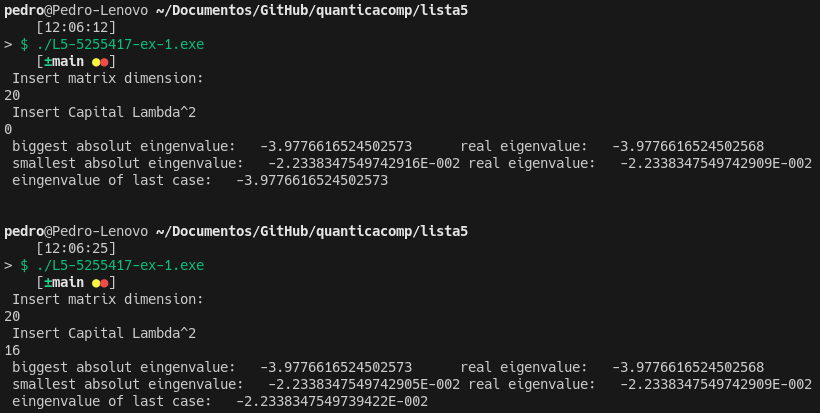
\includegraphics[width=0.8\textwidth]{../images/ex1-20.png}
            \caption{N=20}
        \end{figure}
        \begin{figure}[H]
            \centering
            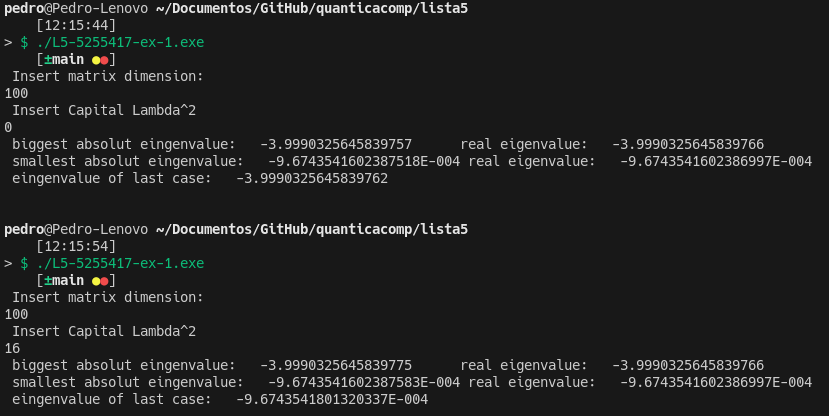
\includegraphics[width=0.8\textwidth]{../images/ex1-100.png}
            \caption{N=100}
        \end{figure}

        Nota-se que o método funcionou, para todos os casos, de acordo com esperado. Em particular, para o caso $\Lambda^2 I - A^2$ v\^e-se que ao escolher $\Lambda$ adequadamente, recupera-se o melhor e o maior autovalores absolutos.
        (O c\'odigo gera um arquivo com os autovetores de cada caso que n\~ao foram colocados no terminal para n\~ao poluir a vizualiza\c{c}\~ao dos resultados)

    \subsection{Exercício 2}

        Considere o poço de potencial infinito para uma partícula de massa $m$, i.e. a equação
        % PDF has \nabla, using \nabla^2 for the Laplacian as is standard.
        $$-\frac{\hbar^{2}}{2m}\nabla^2\psi_{j}(x)=E_{j}\psi_{j}(x) \quad \text{}$$
        Sabemos que no caso de um poço no intervalo $[0, L]$ as autofunções são
        $$ \psi_{j}(x)\propto \sin\left(\frac{j\pi x}{L}\right) \quad \text{}$$
        com autovalores para a energia
        $$ E_{j}=\frac{\hbar^{2}j^{2}\pi^{2}}{2mL^{2}} \quad \text{}$$
        Podemos discretizar a Eq. (1) % Nota: Eq. (1) no texto original é a forma da autofunção. A discretização é da equação de Schrödinger acima.
        usando 
        $$ -2\psi_{m}+\psi_{m+1}+\psi_{m-1}=-\frac{2mE}{\hbar^{2}}\delta x^{2}\psi_{m} \quad \text{}$$
        onde $\delta x=L/(n+1)$ e devemos fixar $\phi_{0}=\phi(0)=0$ e $\phi_{n+1}=\phi(L)=0$. 
        A matriz no lado esquerdo é a matriz $n\times n$ 
        $$
        \begin{pmatrix}
        -2 & 1 & 0 & \cdots & 0 & 0 \\
        1 & -2 & 1 & \cdots & 0 & 0 \\
        0 & 1 & -2 & \cdots & 0 & 0 \\
        \vdots & \vdots & \vdots & \ddots & \vdots & \vdots \\
        0 & 0 & 0 & \cdots & -2 & 1 \\
        0 & 0 & 0 & \cdots & 1 & -2
        \end{pmatrix}
        \quad \text{}
        $$
        aplicada ao vetor $(\psi_{1},\psi_{2},...,\psi_{n-1},\psi_{n})$. De fato, após a multiplicação, a primeira linha é $-2\psi_{1}+\psi_{2},$ que corresponde à expressão $\psi_{0}-2\psi_{1}+\psi_{2}$ com $\psi_{0}=0$. Também, a última linha é $\psi_{n-1}-2\psi_{n},$ que corresponde à expressão $\psi_{n-1}-2\psi_{n}+\psi_{n+1}$ com $\psi_{n+1}=0$. 
        
        Sabemos que para esta matriz os autovalores são $\lambda_{j}=-4\sin^{2}\left[\frac{j\pi}{2(n+2)}\right]$. \quad 
        
        \begin{itemize}
            \item Verifique analiticamente que, no limite de $n\rightarrow+\infty$, os autovalores $\lambda_{j}$ fornecem os autoestados de energia $E_{j}.$ 
            \item Usando o power method calcule a energia do estado fundamental $E_{0}$ com precisão de $10^{-4}$ (compare o resultado com o valor exato). 
            \item Faça um gráfico da autofunção normalizada e compare com a solução exata. 
        \end{itemize}

        O c\'odigo foi compilado com o comando:

    gfortran L5-5255417-ex-2.f90 -Wall -Wextra -pedantic -ffree-form -o L5-5255417-ex-2.exe

            \subsubsection{Demonstra\c{c}\~ao Anal\'itica}

                \textbf{Verificar que:}
                $$-\frac{2mE_j}{\hbar^2}\delta x^2 = -4\sin^2\left[\frac{j\pi}{2(n+1)}\right]$$
                Quando $n \rightarrow \infty$, sabemos que $\delta x = \frac{L}{n+1}$ e a energia converge para $E_j = \frac{\hbar^2j^2\pi^2}{2mL^2}$.

                \vspace{1em}
                \noindent
                \textbf{Expandindo $\sin^2(x)$ em torno de 0:}
                \\
                A aproximação de Taylor para pequenos ângulos é:
                $$\sin^2(x) \approx x^2$$

                \vspace{1em}
                \noindent
                \textbf{Verificação no limite:}
                \\
                Substituindo $E_j$, $\delta x$ e a aproximação do seno na equação inicial:
                $$-\frac{2m}{\hbar^2}\left(\frac{\hbar^2j^2\pi^2}{2mL^2}\right)\left(\frac{L}{n+1}\right)^2 \approx -4\left(\frac{j\pi}{2(n+1)}\right)^2$$
                Simplificando ambos os lados:
                \begin{align*}
                -\frac{2m}{\hbar^2}\frac{\hbar^2j^2\pi^2}{2mL^2}\frac{L^2}{(n+1)^2} &\approx -4\frac{j^2\pi^2}{4(n+1)^2} \\
                -\frac{j^2\pi^2}{(n+1)^2} &= -\frac{j^2\pi^2}{(n+1)^2}
                \end{align*}
                \textbf{Logo,} a relação é válida no limite $n \rightarrow \infty$.

            \subsubsection{Demonstração da Relação entre $\phi(x)$ e $v_i$}

                O objetivo é encontrar a constante de proporcionalidade que relaciona o autovetor discreto $v_i$, obtido numericamente, com a autofunção contínua $\phi(x)$.

                A condição de normalização para a autofunção contínua $\phi(x)$ em um poço de potencial de tamanho $L$ é:
                \begin{equation}
                    \int_{0}^{L} |\phi(x)|^2 \,dx = 1
                \end{equation}

                Podemos aproximar esta integral por uma soma de Riemann sobre $n$ pontos discretos, onde $x_i = i \cdot \delta x$ e $\delta x$ é o passo da discretização:
                \begin{equation}
                    \sum_{i=1}^{n} |\phi(x_i)|^2 \delta x \approx 1
                \end{equation}

                Por outro lado, o autovetor $v$ calculado pelo método numérico é tipicamente normalizado para que a soma de seus componentes ao quadrado seja 1 (norma Euclidiana):
                \begin{equation}
                    \sum_{i=1}^{n} |v_i|^2 = 1
                \end{equation}

                Assumimos que a autofunção nos pontos discretos é proporcional ao autovetor, com uma constante de normalização $C$:
                \begin{equation}
                    \phi(x_i) = C \cdot v_i
                \end{equation}

                Substituindo a equação (4) na equação (2):
                \begin{equation}
                    \sum_{i=1}^{n} |C \cdot v_i|^2 \delta x = 1
                \end{equation}

                Fatorando a constante $C$ e $\delta x$ para fora da soma:
                \begin{equation}
                    C^2 \delta x \sum_{i=1}^{n} |v_i|^2 = 1
                \end{equation}

                Usando a condição de normalização do vetor $v$ da equação (3), a soma se torna 1:
                \begin{align*}
                    C^2 \delta x \cdot (1) &= 1 \\
                    C^2 &= \frac{1}{\delta x} \\
                    C &= \frac{1}{\sqrt{\delta x}}
                \end{align*}

                Portanto, a relação entre a autofunção $\phi$ nos pontos $x_i$ e os componentes do autovetor $v_i$ é:
                \begin{equation}
                    \phi(x_i) = \frac{v_i}{\sqrt{\delta x}}
                \end{equation}
                Esta é a relação utilizada no código para gerar o arquivo de resultados.

        Resultados:

        Utilizou-se N=10000 como se fosse N=infinito, obtendo a energia:
        \begin{figure}[H]
            \centering
            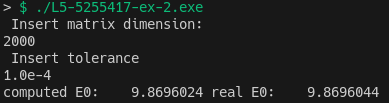
\includegraphics[width=0.8\textwidth]{../images/ex2.png}
        \end{figure}
        E obteve-se a seguinte autofun\c{c}\~ao:
        \begin{figure}[H]
            \centering
            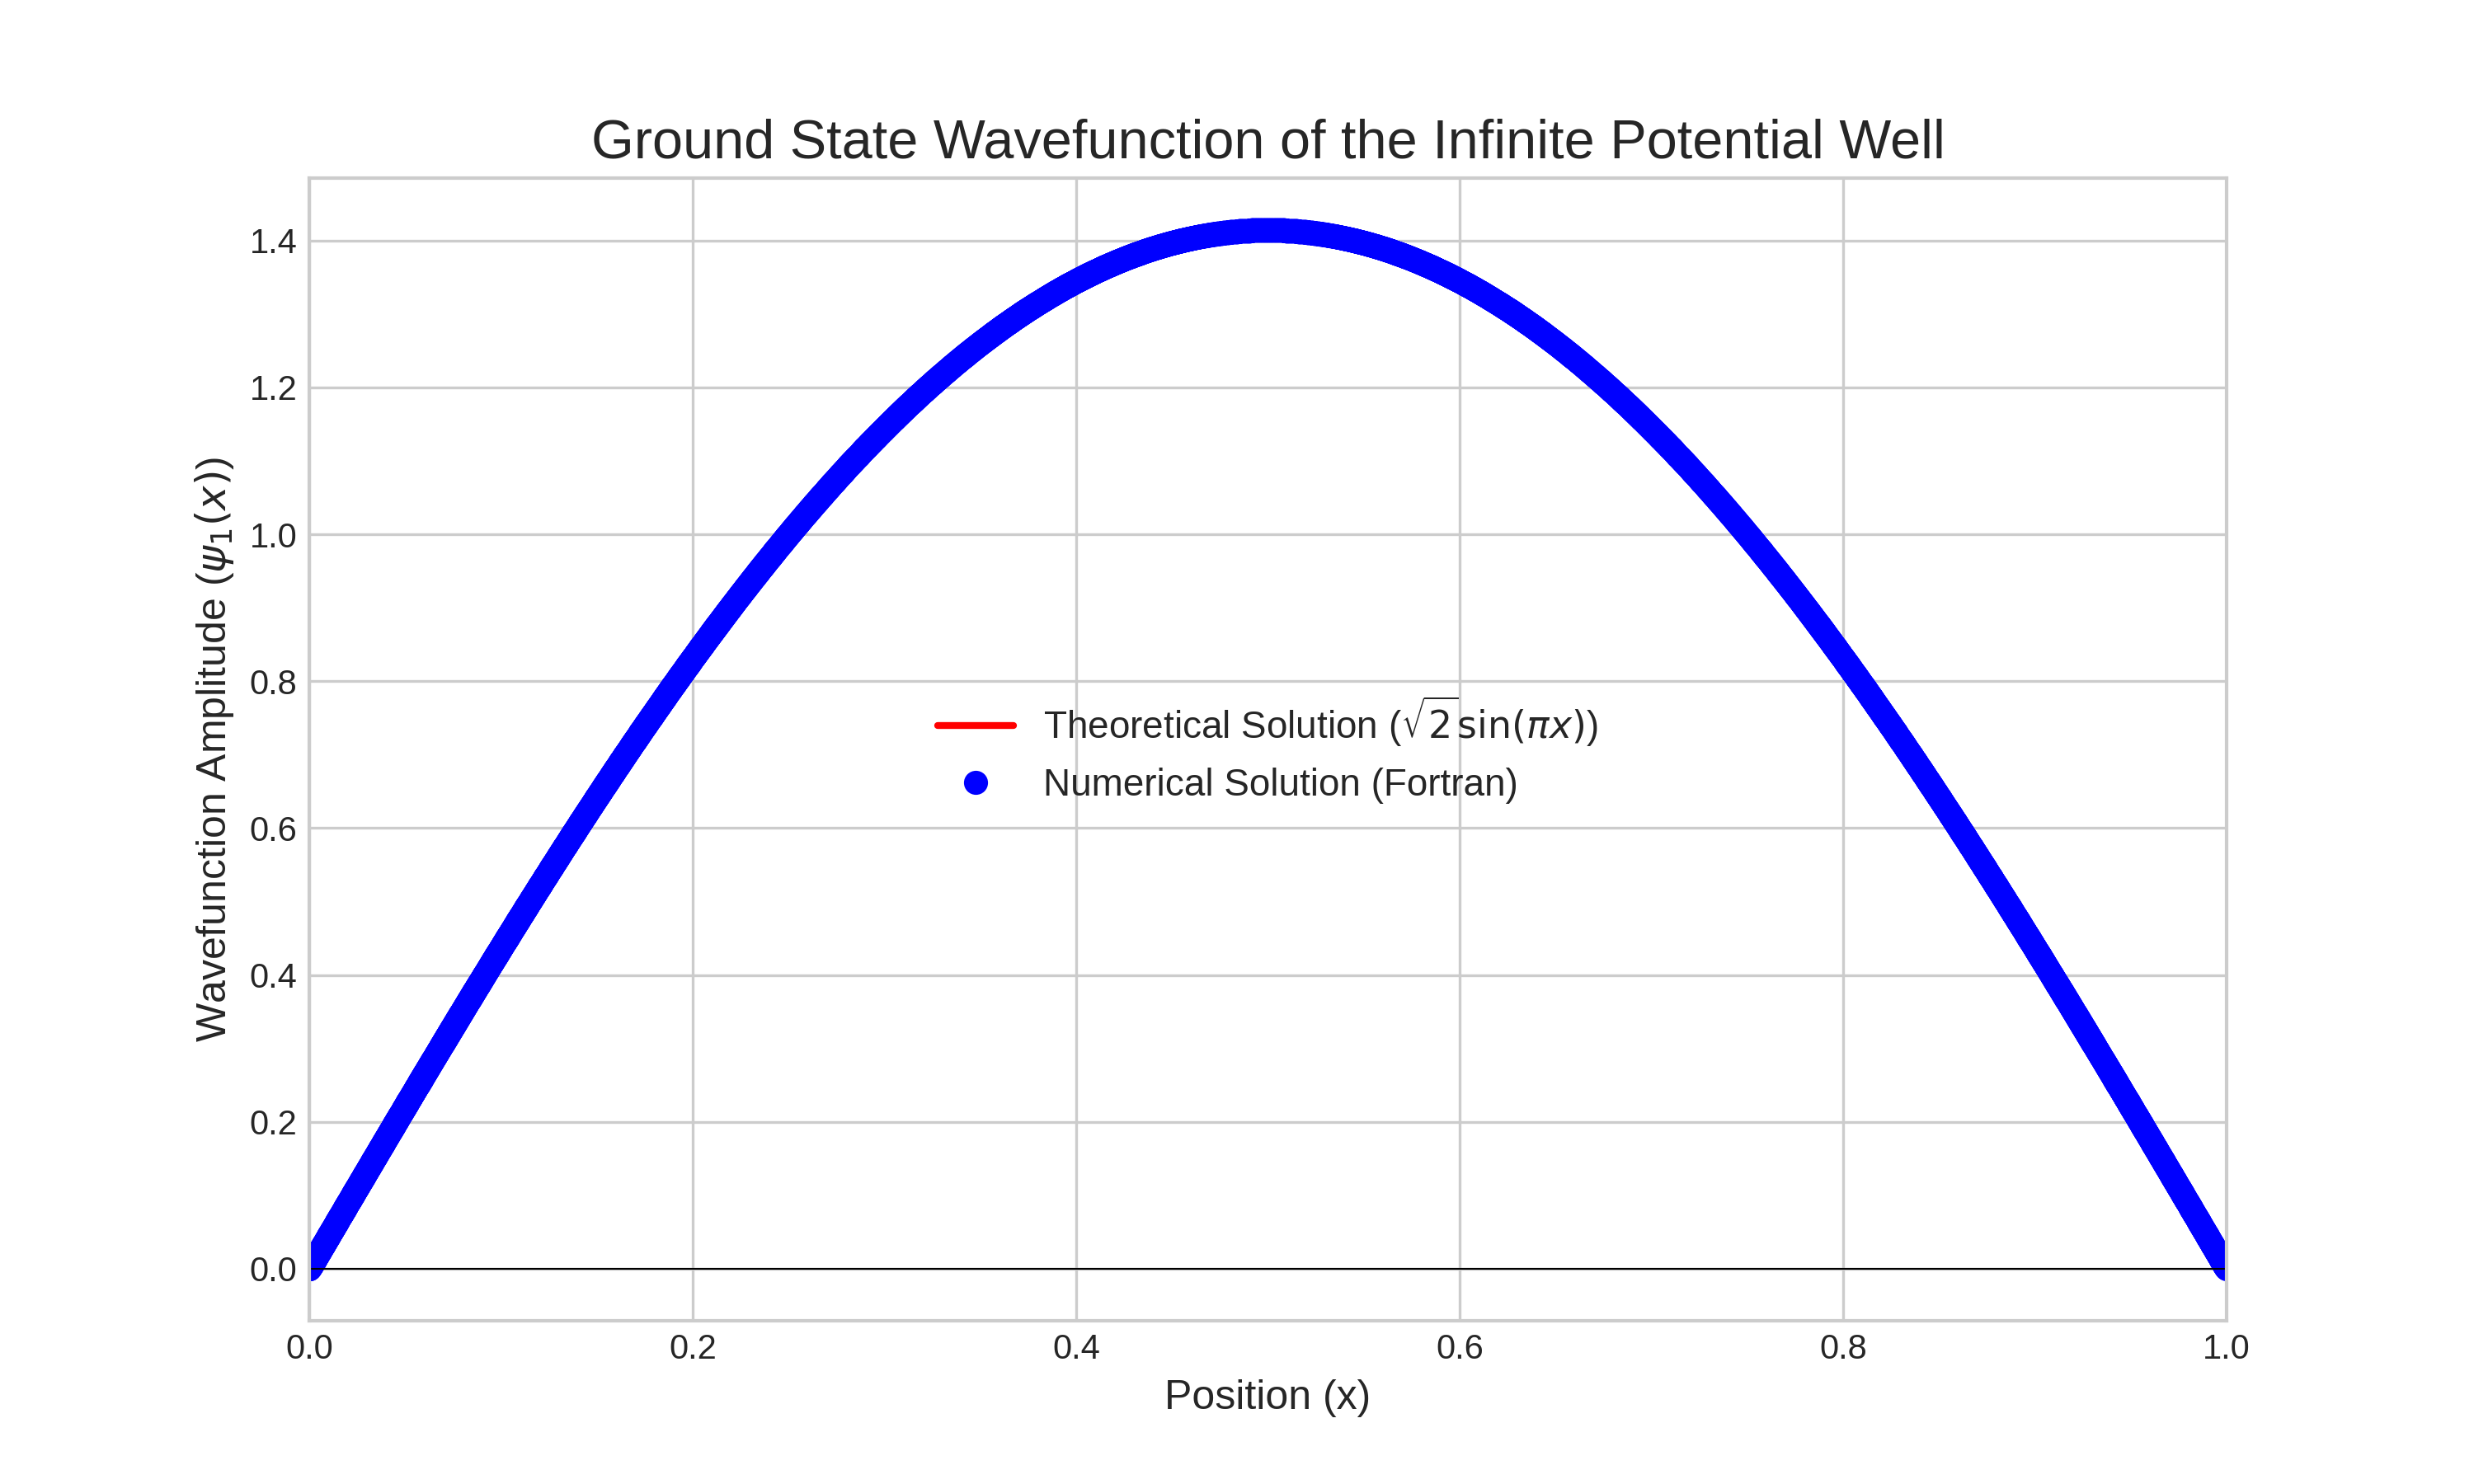
\includegraphics[width=0.8\textwidth]{../images/wavefunction_plot.png}
        \end{figure}

    De modo que corresponde perfeitamente à fun\c{c}\~ao conhecida
        

\end{document}